% Provenance (never printed): cycle 4 (geographie and SVT, "La planete Terre"):
% why a flat map distorts, projections, scale, topographic maps and
% profiles, satellite images and satellite positioning; see
% sources/book1/PROVENANCE.md. Book 1, grade 9, chapter 5.
% Vocabulary guard: owns map projection (Mercator, equal-area), numerical
% scale and scale bar, topographic map, contour line and contour interval,
% remote sensing and satellite image, satellite positioning. "Scale" itself
% is g2's (drawing-to-map, Sync 1 ruling); globe and world map are g3's;
% parallels, meridians, latitude and longitude are g6's; altitude, relief
% and physical map are g4's; slope as a percentage was used in g9.2. The
% speed of light is the physics books' (recalled in prose). The V-rule of
% geological maps belongs to Book 3.
\chapter{पूरी पृथ्वी के मानचित्र}\label{ch:g9:maps-of-the-earth}

कक्षा की दीवार पर टँगे कई \omterm{def:g2:drawing-to-map:map}{मानचित्रों} पर ग्रीनलैंड लगभग अफ़्रीका जितना बड़ा दिखता है। \omterm{def:g3:continents-and-oceans:globe}{ग्लोब} पर
अफ़्रीका लगभग चौदह गुना बड़ा है: अफ़्रीका की मुख्य भूमि के लिए लगभग 29~मिलियन वर्ग किलोमीटर,
जबकि ग्रीनलैंड के लिए लगभग 2.1~मिलियन। दोनों पृथ्वी के सच्चे चित्र हैं, सावधानी से बनाए
गए। तो कौन-सा झूठ बोल रहा है, और क्यों?
% ledger: data:ne-land (areas computed in figdata/grade-9/projections.py)

\begin{recall}
\omterm{def:g2:drawing-to-map:map}{मानचित्र} ऊपर से देखी गई किसी जगह का चित्र है, उस जगह से छोटा, \omterm{def:g2:drawing-to-map:legend}{संकेत-सूची} और \omterm{def:g2:drawing-to-map:scale}{मापनी} के साथ
(\cref{ch:g2:drawing-to-map})। \omterm{def:g3:continents-and-oceans:globe}{ग्लोब} गोल पृथ्वी का एक छोटा मॉडल है; \omterm{def:g3:continents-and-oceans:world-map}{विश्व मानचित्र} पूरी
पृथ्वी को चपटी, एक ही चित्र में दिखाता है (\cref{ch:g3:continents-and-oceans})। \omterm{def:g6:latitude-longitude:latitude}{अक्षांश
रेखाएँ} और \omterm{def:g6:latitude-longitude:longitude}{याम्योत्तर} हर जगह को उसका \omterm{def:g6:latitude-longitude:latitude}{अक्षांश} और \omterm{def:g6:latitude-longitude:longitude}{देशांतर} देते हैं
(\cref{ch:g6:latitude-longitude})। ऊँचाई \omterm{def:g4:world-physical-map:altitude}{समुद्र तल} से ऊपर की ऊँचाई है, और \omterm{def:g4:world-physical-map:physical-map}{भौतिक मानचित्र}
\omterm{def:g4:world-physical-map:relief}{उच्चावच} को रंगों में दिखाता है (\cref{ch:g4:world-physical-map})। भौतिकी में तुम सीखते हो
कि प्रकाश लगभग \qty{300000}{km} प्रति सेकंड की चाल से चलता
है।
\end{recall}
% ledger: const:c

\section{चपटे मानचित्र को विकृत क्यों करना पड़ता है}

किसी संतरे के छिलके को मेज़ पर चपटा करके देखो: वह फट जाता है या खिंच जाता है। किसी गोले की
सतह को कुछ लंबाइयाँ बदले बिना चपटा नहीं बिछाया जा सकता। पूरी पृथ्वी को एक काग़ज़ पर बनाने के
लिए मानचित्रकार एक ऐसा नियम चुनता है जो \omterm{def:g3:continents-and-oceans:globe}{ग्लोब} के हर बिंदु को काग़ज़ के एक बिंदु तक भेजता है,
और चुनता है कि \omterm{def:g2:drawing-to-map:map}{मानचित्र} क्या सच रखेगा, और क्या छोड़
देगा।

\begin{definition}[मानचित्र प्रक्षेप]\label{def:g9:maps-of-the-earth:projection}
\emph{मानचित्र प्रक्षेप}\index{मानचित्र प्रक्षेप} एक ऐसा नियम है जो \omterm{def:g3:continents-and-oceans:globe}{ग्लोब} के हर बिंदु को,
उसके \omterm{def:g6:latitude-longitude:latitude}{अक्षांश} और \omterm{def:g6:latitude-longitude:longitude}{देशांतर} से दिए गए, एक चपटे \omterm{def:g2:drawing-to-map:map}{मानचित्र} के एक बिंदु तक भेजता है।
\emph{मर्केटर प्रक्षेप}\index{मर्केटर प्रक्षेप} पर \omterm{def:g6:latitude-longitude:latitude}{अक्षांश रेखाएँ} और \omterm{def:g6:latitude-longitude:longitude}{याम्योत्तर} समकोण पर
काटती सीधी रेखाएँ होते हैं, और हर छोटे क्षेत्र का आकार बना रहता है, पर \omterm{def:g3:continents-and-oceans:poles}{ध्रुवों} की ओर क्षेत्रफल
और ज़्यादा बढ़ाए जाते हैं। \emph{समक्षेत्र
प्रक्षेप}\index{समक्षेत्र प्रक्षेप} पर हर क्षेत्र दूसरों की तुलना में अपना सच्चा क्षेत्रफल
रखता है, पर आकार मुड़ जाते हैं, \omterm{def:g2:drawing-to-map:map}{मानचित्र} के किनारों की ओर और
ज़्यादा।
\end{definition}

नीचे का चित्र \omterm{def:g3:continents-and-oceans:globe}{ग्लोब} पर बने एक जैसे वृत्तों को, सभी एक ही आकार के, दोनों \omterm{def:g2:drawing-to-map:map}{मानचित्रों} पर
बनाता है। मर्केटर \omterm{def:g2:drawing-to-map:map}{मानचित्र} पर वृत्त गोल रहते हैं पर \omterm{def:g3:continents-and-oceans:poles}{ध्रुवों} की ओर बढ़ते जाते हैं: \omterm{def:g6:latitude-longitude:latitude}{अक्षांश}
\ang{60} पर उनका क्षेत्रफल \omterm{def:g3:continents-and-oceans:equator}{भूमध्य रेखा} वाले का चार गुना है, और ग्रीनलैंड के बीच के पास,
लगभग \ang{72} पर, लगभग दस गुना। समक्षेत्र \omterm{def:g2:drawing-to-map:map}{मानचित्र} पर सभी वृत्त एक ही क्षेत्रफल रखते हैं,
पर केंद्र से दूर वाले दबकर अंडाकार हो जाते हैं।
% ledger: data:ne-land (circles and factors computed in figdata/grade-9/projections.py, mercator_area_factor)

कोई भी प्रक्षेप हर चीज़ के लिए सबसे अच्छा नहीं है। \omterm{def:g9:maps-of-the-earth:projection}{मर्केटर प्रक्षेप} नाविकों के लिए बनाया गया
था: जो मार्ग कम्पास की एक ही दिशा बनाए रखता है, वह उस पर एक सीधी रेखा है। देशों, जंगलों या
\omterm{def:g5:weather-and-climate:desert}{मरुस्थलों} के आकारों की तुलना करने के लिए समक्षेत्र \omterm{def:g2:drawing-to-map:map}{मानचित्र} सच बताता है। किसी \omterm{def:g3:continents-and-oceans:world-map}{विश्व मानचित्र}
पर भरोसा करने से पहले यह पूछना ठीक है कि वह कौन-सा प्रक्षेप इस्तेमाल करता
है।

\begin{omfigure}
\begin{tikzpicture}
\begin{axis}[name=merc, x=0.0215cm, y=0.0215cm, xmin=-180, xmax=180,
  ymin=-140, ymax=169, axis line style={black!50}, ticks=none,
  title={\footnotesize मर्केटर प्रक्षेप}, title style={yshift=-1ex}]
  \addplot[black!15, line width=0.3pt] table {figdata/out/grade-9-projections-merc-grid.dat};
  \addplot[fill=black!25, draw=black!45, line width=0.15pt] table {figdata/out/grade-9-projections-merc-land.dat};
  \addplot[fill=orange!55, draw=orange!70!black, line width=0.3pt] table {figdata/out/grade-9-projections-merc-greenland.dat};
  \addplot[fill=blue!30, draw=blue!60!black, line width=0.3pt] table {figdata/out/grade-9-projections-merc-africa.dat};
  \addplot[red!80!black, line width=0.6pt] table {figdata/out/grade-9-projections-merc-circles.dat};
\end{axis}
\begin{axis}[at={(merc.east)}, anchor=west, xshift=0.3cm, x=0.025cm, y=0.025cm,
  xmin=-165, xmax=165, ymin=-83, ymax=83, hide axis,
  title={\footnotesize एक समक्षेत्र प्रक्षेप}, title style={yshift=-1ex}]
  \addplot[black!15, line width=0.3pt] table {figdata/out/grade-9-projections-moll-grid.dat};
  \addplot[fill=black!25, draw=black!45, line width=0.15pt] table {figdata/out/grade-9-projections-moll-land.dat};
  \addplot[fill=orange!55, draw=orange!70!black, line width=0.3pt] table {figdata/out/grade-9-projections-moll-greenland.dat};
  \addplot[fill=blue!30, draw=blue!60!black, line width=0.3pt] table {figdata/out/grade-9-projections-moll-africa.dat};
  \addplot[red!80!black, line width=0.6pt] table {figdata/out/grade-9-projections-moll-circles.dat};
\end{axis}
\end{tikzpicture}

{\small एक ही दुनिया दो प्रक्षेपों पर। लाल: \omterm{def:g3:continents-and-oceans:globe}{ग्लोब} पर एक ही आकार के वृत्त, \omterm{def:g6:latitude-longitude:latitude}{अक्षांश} के
हर \ang{30} और \omterm{def:g6:latitude-longitude:longitude}{देशांतर} के हर \ang{60} पर केंद्रित। नारंगी: ग्रीनलैंड; नीला: अफ़्रीका की
मुख्य भूमि। मर्केटर \omterm{def:g2:drawing-to-map:map}{मानचित्र} पर (बाएँ, \ang{80} दक्षिण और \ang{84} उत्तर पर काटा गया,
क्योंकि \omterm{def:g3:continents-and-oceans:poles}{ध्रुव} अनंत दूरी पर होते), दोनों लगभग एक ही आकार के दिखते हैं; समक्षेत्र \omterm{def:g2:drawing-to-map:map}{मानचित्र} पर
(दाएँ), अफ़्रीका लगभग 14 गुना बड़ा है, जैसा \omterm{def:g3:continents-and-oceans:globe}{ग्लोब} पर। तटरेखाएँ नेचुरल अर्थ
से।}
% ledger: data:ne-land
\label{fig:g9:maps-of-the-earth:projections}
\end{omfigure}

\begin{example}[ग्रीनलैंड और अफ़्रीका]
अफ़्रीका की मुख्य भूमि लगभग 29~मिलियन~\unit{km^2} घेरती है, ग्रीनलैंड लगभग
2.1~मिलियन~\unit{km^2}: $29 \div 2.1 \approx 14$। अफ़्रीका \omterm{def:g3:continents-and-oceans:equator}{भूमध्य रेखा} के दोनों ओर
फैला है, जहाँ \omterm{def:g9:maps-of-the-earth:projection}{मर्केटर प्रक्षेप} मुश्किल से कुछ बढ़ाता है, जबकि ग्रीनलैंड का ज़्यादातर हिस्सा लगभग
\ang{60} और \ang{84} उत्तर के बीच है, जहाँ क्षेत्रफल 4 से 10 से ज़्यादा गुना तक बढ़ाए जाते
हैं। मर्केटर \omterm{def:g2:drawing-to-map:map}{मानचित्र} पर दोनों लगभग एक ही आकार के निकलते
हैं।
\end{example}
% ledger: data:ne-land (areas and ratios computed in figdata/grade-9/projections.py, areas)

\section{मापनी}

किसी \omterm{def:g1:landscapes-around-us:landform}{घाटी} या कस्बे का \omterm{def:g2:drawing-to-map:map}{मानचित्र} पृथ्वी का इतना छोटा टुकड़ा है कि प्रक्षेप से मुश्किल से फ़र्क़
पड़ता है। जो मायने रखता है वह यह है कि \omterm{def:g2:drawing-to-map:map}{मानचित्र} ज़मीन से कितना छोटा
है।

\begin{definition}[संख्यात्मक मापनी और मापनी-पट्टी]\label{def:g9:maps-of-the-earth:numerical-scale}
किसी \omterm{def:g2:drawing-to-map:map}{मानचित्र} की \emph{संख्यात्मक मापनी}\index{संख्यात्मक मापनी} एक अनुपात है जैसे
$1 : 25\,000$: \omterm{def:g2:drawing-to-map:map}{मानचित्र} पर एक सेंटीमीटर ज़मीन पर \num{25000} सेंटीमीटर दिखाता है, और
किसी भी इकाई के लिए यही। \emph{मापनी-पट्टी}\index{मापनी-पट्टी} \omterm{def:g2:drawing-to-map:map}{मानचित्र} पर बना एक
पैमाना है, जिस पर ज़मीन की दूरियाँ अंकित होती
हैं।
\end{definition}

\begin{method}[संख्यात्मक मापनी का उपयोग]
\begin{enumerate}
  \item \omterm{def:g2:drawing-to-map:map}{मानचित्र} पर दूरी सेंटीमीटर में मापो।
  \item उसे कोलन के बाद वाली संख्या से गुणा करो: नतीजा ज़मीन पर दूरी है,
        सेंटीमीटर में।
  \item बदलो: मीटर के लिए 100 से भाग दो, किलोमीटर के लिए \num{100000} से।
\end{enumerate}
\end{method}

\begin{example}[$1 : 25\,000$ के मानचित्र पर एक सैर]
$1 : 25\,000$ के \omterm{def:g2:drawing-to-map:map}{मानचित्र} पर एक पगडंडी \qty{6}{cm} मापती है। ज़मीन पर
वह $6 \times 25\,000 = \num{150000}$~cm है, यानी \qty{1500}{m} या
\qty{1.5}{km}। \omterm{def:g2:drawing-to-map:map}{मानचित्र} का हर सेंटीमीटर \qty{250}{m} दिखाता है।
\end{example}

\omterm{def:g9:maps-of-the-earth:numerical-scale}{मापनी-पट्टी} का \omterm{def:g9:maps-of-the-earth:numerical-scale}{संख्यात्मक मापनी} पर एक फ़ायदा है: जब कोई \omterm{def:g2:drawing-to-map:map}{मानचित्र} स्क्रीन पर या कॉपी मशीन
से बड़ा या छोटा किया जाता है, तो पट्टी भी उसके साथ बड़ी या छोटी होती है और सही रहती है, जबकि
कोने में छपा अनुपात ग़लत हो जाता
है।

\section{स्थलाकृतिक मानचित्र}

\omterm{def:g4:world-physical-map:physical-map}{भौतिक मानचित्र} \omterm{def:g4:world-physical-map:relief}{उच्चावच} को रंगों से दिखाता है। किसी छोटे इलाक़े का \omterm{def:g2:drawing-to-map:map}{मानचित्र} उसे कहीं ज़्यादा
सटीकता से, रेखाओं से, दिखाता है।

\begin{definition}[स्थलाकृतिक मानचित्र]\label{def:g9:maps-of-the-earth:topographic-map}
\emph{स्थलाकृतिक मानचित्र}\index{स्थलाकृतिक मानचित्र} किसी छोटे इलाक़े का एक विस्तृत
\omterm{def:g2:drawing-to-map:map}{मानचित्र} है, $1 : 25\,000$ या $1 : 50\,000$ जैसी \omterm{def:g2:drawing-to-map:scale}{मापनी} पर, जो \omterm{def:g1:landscapes-around-us:water}{नदियों}, सड़कों,
रास्तों, इमारतों और जंगलों के साथ ज़मीन का आकार और ऊँचाई दिखाता
है।
\end{definition}

\begin{definition}[समोच्च रेखा और समोच्च अंतराल]\label{def:g9:maps-of-the-earth:contour}
\emph{समोच्च रेखा}\index{समोच्च रेखा} \omterm{def:g2:drawing-to-map:map}{मानचित्र} पर एक ऐसी रेखा है जो ज़मीन के एक ही
ऊँचाई वाले बिंदुओं को जोड़ती है। \emph{समोच्च
अंतराल}\index{समोच्च अंतराल} दो पड़ोसी समोच्च रेखाओं के बीच ऊँचाई का अंतर है; वह पूरे
\omterm{def:g2:drawing-to-map:map}{मानचित्र} पर एक ही होता है।
\end{definition}

किसी \omterm{def:g1:landscapes-around-us:landform}{पहाड़ी} की कल्पना करो जिसे क्षैतिज तलों से काटा गया है, हर \qty{100}{m} पर एक। हर
कटान \omterm{def:g1:landscapes-around-us:landform}{पहाड़ी} को एक बंद रेखा के साथ काटता है; ऊपर से देखने पर ये रेखाएँ \omterm{def:g9:maps-of-the-earth:contour}{समोच्च रेखाएँ}
हैं।

\begin{omfigure}
\begin{tikzpicture}[font=\footnotesize]
  % side view
  \fill[black!13] (0,0) .. controls (1.2,0.3) and (2.0,1.3) .. (2.8,2.2)
     .. controls (3.2,2.6) and (3.5,2.6) .. (3.7,2.2) .. controls (3.9,1.6) and (4.1,0.4) .. (4.5,0) -- cycle;
  \draw[black!70] (0,0) .. controls (1.2,0.3) and (2.0,1.3) .. (2.8,2.2)
     .. controls (3.2,2.6) and (3.5,2.6) .. (3.7,2.2) .. controls (3.9,1.6) and (4.1,0.4) .. (4.5,0);
  \draw[black!70] (-0.3,0) -- (4.9,0);
  \foreach \y/\h in {0.6/100, 1.2/200, 1.8/300} {
    \draw[omContour, dashed] (-0.3,\y) -- (4.9,\y);
    \node[anchor=east, omContour] at (-0.3,\y) {\h~m};
  }
  \node[anchor=south] at (3.3,2.5) {बगल से देखा गया};
  \node[anchor=north] at (1.4,-0.05) {हल्की पश्चिमी ढाल};
  \node[anchor=north] at (4.1,-0.05) {खड़ी पूर्वी ढाल};
  % map view
  \begin{scope}[xshift=8.4cm, yshift=1.3cm]
    \draw[omContour, line width=0.5pt] (0.25,0) ellipse (2.1 and 1.25);
    \draw[omContour, line width=0.5pt] (0.75,0.02) ellipse (1.3 and 0.9);
    \draw[omContour, line width=0.5pt] (1.05,0.04) ellipse (0.62 and 0.5);
    \fill (1.25,0.05) circle (0.04);
    \draw[black!60] (1.25,0.05) -- (2.9,-0.6) node[anchor=west, inner sep=1.5pt] {शिखर};
    \node[omContour, fill=white, inner sep=0.5pt] at (-1.85,0) {100};
    \node[omContour, fill=white, inner sep=0.5pt] at (-0.55,0) {200};
    \node[omContour, fill=white, inner sep=0.5pt] at (0.43,0) {300};
    \node[anchor=north] at (0.25,-1.35) {ऊपर से देखा गया: समोच्च रेखाएँ};
    \draw[->] (2.7,0.9) -- (2.7,1.4) node[above] {उ};
  \end{scope}
\end{tikzpicture}

{\small हर \qty{100}{m} पर काटी गई एक \omterm{def:g1:landscapes-around-us:landform}{पहाड़ी} (एक रेखाचित्र)। ऊपर से देखने पर हर कटान
शिखर के चारों ओर एक बंद \omterm{def:g9:maps-of-the-earth:contour}{समोच्च रेखा} देता है। जहाँ ढाल खड़ी है (पूर्व), वहाँ रेखाएँ पास-पास हैं;
जहाँ हल्की है (पश्चिम), वहाँ वे दूर-दूर
हैं।}
\label{fig:g9:maps-of-the-earth:slices}
\end{omfigure}

\omterm{def:g9:maps-of-the-earth:topographic-map}{स्थलाकृतिक मानचित्र} कुछ नियमों से पढ़ा जाता है।
\begin{itemize}
  \item \omterm{def:g9:maps-of-the-earth:contour}{समोच्च रेखाएँ} कभी एक-दूसरे को नहीं काटतीं: किसी बिंदु की केवल एक ऊँचाई होती है।
  \item \omterm{def:g9:maps-of-the-earth:contour}{समोच्च रेखाएँ} जितनी पास-पास, ढाल उतनी खड़ी; दूर-दूर हों तो ज़मीन हल्की ढाल वाली है;
        कोई रेखा ही न हो तो वह लगभग समतल है।
  \item एक-दूसरे के अंदर बनी बंद रेखाएँ, जो अंदर की ओर ऊँची होती जाएँ, किसी \omterm{def:g1:landscapes-around-us:landform}{पहाड़ी} को
        दिखाती हैं; उसकी चोटी अक्सर अपनी ऊँचाई के साथ एक बिंदु से चिह्नित होती है, एक
        \emph{स्थानिक ऊँचाई}।
  \item जहाँ कोई \omterm{def:g9:maps-of-the-earth:contour}{समोच्च रेखा} किसी \omterm{def:g1:landscapes-around-us:landform}{घाटी} को पार करती है, वहाँ वह धारा की उलटी दिशा में मुड़ती
        है, एक V के आकार में जिसकी नोक \omterm{def:g1:landscapes-around-us:landform}{घाटी} के सिरे की ओर होती है।
  \item हर पाँचवीं रेखा, \emph{सूचक \omterm{def:g9:maps-of-the-earth:contour}{समोच्च रेखा}}, मोटी बनाई जाती है और उस पर उसकी
        ऊँचाई लिखी होती है।
\end{itemize}

दो बिंदुओं के बीच ज़मीन की ढाल उठाव को क्षैतिज दूरी से भाग देने पर मिलती है, जिसे अक्सर
प्रतिशत में लिखा जाता है। नीचे के \omterm{def:g2:drawing-to-map:map}{मानचित्र} पर, \omterm{def:g1:landscapes-around-us:water}{नदी} से उत्तर की ओर जाते हुए, रेखा C--D पर
\qty{200}{m} और \qty{400}{m} की \omterm{def:g9:maps-of-the-earth:contour}{समोच्च रेखाएँ} लगभग \qty{0.75}{km} दूर हैं: ढाल लगभग
$200 \div 750
\approx 0.27$, या \qty{27}{\%}
है।
% ledger: (invented region: crossings 2.09 and 2.83 km from C, figdata/grade-9/varden_topo.py)

\begin{method}[स्थलाकृतिक परिच्छेदिका बनाना]
\begin{enumerate}
  \item \omterm{def:g2:drawing-to-map:map}{मानचित्र} पर परिच्छेदिका की रेखा बनाओ, एक सिरे (C) से दूसरे सिरे
        (D) तक।
  \item काग़ज़ की एक पट्टी का सीधा किनारा रेखा के साथ रखो; C, D, और हर वह बिंदु चिह्नित
        करो जहाँ रेखा किसी \omterm{def:g9:maps-of-the-earth:contour}{समोच्च रेखा} को काटती है, उसकी ऊँचाई के
        साथ।
  \item C--D जितना लंबा एक क्षैतिज अक्ष (दूरियाँ) और ऊँचाइयों का एक ऊर्ध्वाधर अक्ष
        बनाओ।
  \item हर निशान को ग्राफ़ पर ले जाओ, C से उसकी दूरी पर और उसकी ऊँचाई पर, और बिंदुओं
        को एक चिकने वक्र से जोड़ो: \omterm{def:g1:landscapes-around-us:landform}{पहाड़ियों} की चोटियों पर गोल, \omterm{def:g1:landscapes-around-us:landform}{घाटी} के तल के साथ
        समतल।
\end{enumerate}
\end{method}

\begin{omfigure}
\begin{tikzpicture}
\begin{axis}[name=map, x=2cm, y=2cm, xmin=2, xmax=8, ymin=1.8, ymax=6.2, ticks=none,
  axis line style={black!60}, clip mode=individual]
  \addplot[contour] table {figdata/out/shared-region-contours.dat};
  \addplot[index contour] table {figdata/out/shared-region-index-contours.dat};
  \addplot[river] table {figdata/out/shared-region-river.dat};
  \addplot[only marks, mark=none, point meta=explicit symbolic, nodes near coords,
    nodes near coords align={center}, nodes near coords style={font=\tiny, fill=white, inner sep=0.6pt, text=omContour}]
    table[meta=label] {figdata/out/grade-9-varden_topo-labels.dat};
  \addplot[only marks, mark=*, mark size=1.2pt, point meta=explicit symbolic, nodes near coords,
    nodes near coords align={right}, nodes near coords style={font=\scriptsize, inner sep=1.5pt}]
    table[meta=label] {figdata/out/grade-9-varden_topo-spots.dat};
  \addplot[black, line width=0.8pt] table[x=x_km, y=y_km] {figdata/out/grade-9-varden_topo-cd.dat};
  \addplot[only marks, mark=none, point meta=explicit symbolic, nodes near coords,
    nodes near coords align={left}, nodes near coords style={font=\small\bfseries, inner sep=2pt}]
    table[meta=label] {figdata/out/grade-9-varden_topo-cd.dat};
  \coordinate (na) at (axis cs:8.3,5.3);
  \coordinate (sb) at (axis cs:2.2,1.95);
\end{axis}
\pic at (na) {northarrow};
\fill[white] ($(sb)+(-0.1,-0.42)$) rectangle ($(sb)+(2.3,0.25)$);
\pic at (sb) {scalebar={2}{1 km}};
\node[anchor=west, font=\footnotesize, fill=white, inner sep=1pt] at ($(sb)+(2.35,0.06)$) {$1 : 50\,000$};
\begin{axis}[at={(map.south)}, anchor=north, yshift=-0.9cm, x=2cm, y=0.006cm, clip=false,
  xmin=0, xmax=4, ymin=100, ymax=600, axis x line=bottom, axis y line=left,
  axis line style={-}, grid=major, grid style={black!12},
  xtick={0,1,2,3,4}, ytick={100,200,...,600}, tick label style={font=\scriptsize},
  xlabel={C से दूरी (km)}, ylabel={ऊँचाई (m)}, label style={font=\footnotesize}]
  \addplot[black!70, line width=0.8pt] table[x=s_km, y=z_m] {figdata/out/grade-9-varden_topo-profile.dat};
  \addplot[only marks, mark=*, mark size=1.1pt, omContour] table[x=s_km, y=z_m] {figdata/out/grade-9-varden_topo-cross.dat};
  \node[font=\small\bfseries, anchor=south] at (axis cs:0,600) {C};
  \node[font=\small\bfseries, anchor=south] at (axis cs:4,600) {D};
\end{axis}
\end{tikzpicture}

{\small ऊपर: वार्डन पहाड़ियों के एक हिस्से का $1 : 50\,000$ पर \omterm{def:g9:maps-of-the-earth:topographic-map}{स्थलाकृतिक मानचित्र}
(\omterm{def:g2:drawing-to-map:map}{मानचित्र} पर 1~cm ज़मीन पर \qty{500}{m} के लिए)। \omterm{def:g9:maps-of-the-earth:contour}{समोच्च अंतराल} \qty{50}{m}; सूचक
\omterm{def:g9:maps-of-the-earth:contour}{समोच्च रेखाएँ}, ज़्यादा मोटी, 250 और \qty{500}{m} पर हैं। \omterm{def:g1:landscapes-around-us:water}{नदी} एक समतल \omterm{def:g1:landscapes-around-us:landform}{घाटी} तल के साथ
पूर्व की ओर बहती है। नीचे: C--D के साथ स्थलाकृतिक परिच्छेदिका, दक्षिण से उत्तर; बिंदु वे
जगहें हैं जहाँ C--D किसी \omterm{def:g9:maps-of-the-earth:contour}{समोच्च रेखा} को काटती है (ऊर्ध्वाधर मापनी तीन गुना खींची गई
है)।}
% ledger: (invented region: the Varden Hills, figdata/shared/region.py; labels, spot height and profile from figdata/grade-9/varden_topo.py)
\label{fig:g9:maps-of-the-earth:topo}
\end{omfigure}

\section{पृथ्वी के उपग्रह चित्र}

23~जुलाई 1972 को एक रॉकेट ने पृथ्वी की सतह का अध्ययन करने के लिए बनाया गया पहला उपग्रह
छोड़ा, जिसे बाद में लैंडसैट~1 कहा गया। \qty{917}{km} की ऊँचाई पर, \omterm{def:g3:continents-and-oceans:poles}{ध्रुव} से \omterm{def:g3:continents-and-oceans:poles}{ध्रुव} तक,
दिन में 14 बार पृथ्वी की परिक्रमा करते हुए, वह हर 18 दिनों पर उसी जगह के ऊपर से गुज़रता था
और छह वर्षों में उसने पृथ्वी की सतह के लगभग तीन चौथाई हिस्से के चित्र लिए। तब से लैंडसैट
उपग्रह बिना रुके ज़मीन के चित्र लेते आ रहे
हैं।
% ledger: usgs:landsat1

\begin{definition}[सुदूर संवेदन और उपग्रह चित्र]\label{def:g9:maps-of-the-earth:remote-sensing}
\emph{सुदूर संवेदन}\index{सुदूर संवेदन} दूरी से, विमानों से या उपग्रहों से, पृथ्वी का
प्रेक्षण है, उस प्रकाश और दूसरे विकिरण को मापकर जो सतह वापस भेजती है। \emph{उपग्रह
चित्र}\index{उपग्रह चित्र} इन मापों से बना पृथ्वी के किसी हिस्से का एक
चित्र
है।
\end{definition}

उपग्रह का कैमरा हमारी आँखों से ज़्यादा देखता है: वह अवरक्त प्रकाश भी मापता है, जो अदृश्य है।
चित्र पर रंगों में दिखाया गया (एक \emph{छद्म-रंग} चित्र), अवरक्त पौधों, गीली ज़मीन या नंगी
\omterm{def:g3:stones-pebbles-sand:rock}{चट्टान} को उजागर करता है। वर्षों के अंतर पर ली गई एक ही जगह की तस्वीरें दिखाती हैं कि कोई \omterm{def:g1:landscapes-around-us:water}{तट},
जंगल, \omterm{def:g8:ice-on-earth:glacier}{हिमनद} या कस्बा कैसे बदलता है
(\cref{ch:g8:ice-on-earth})।

\begin{omfigure}
\begin{minipage}[c]{0.5\linewidth}\centering
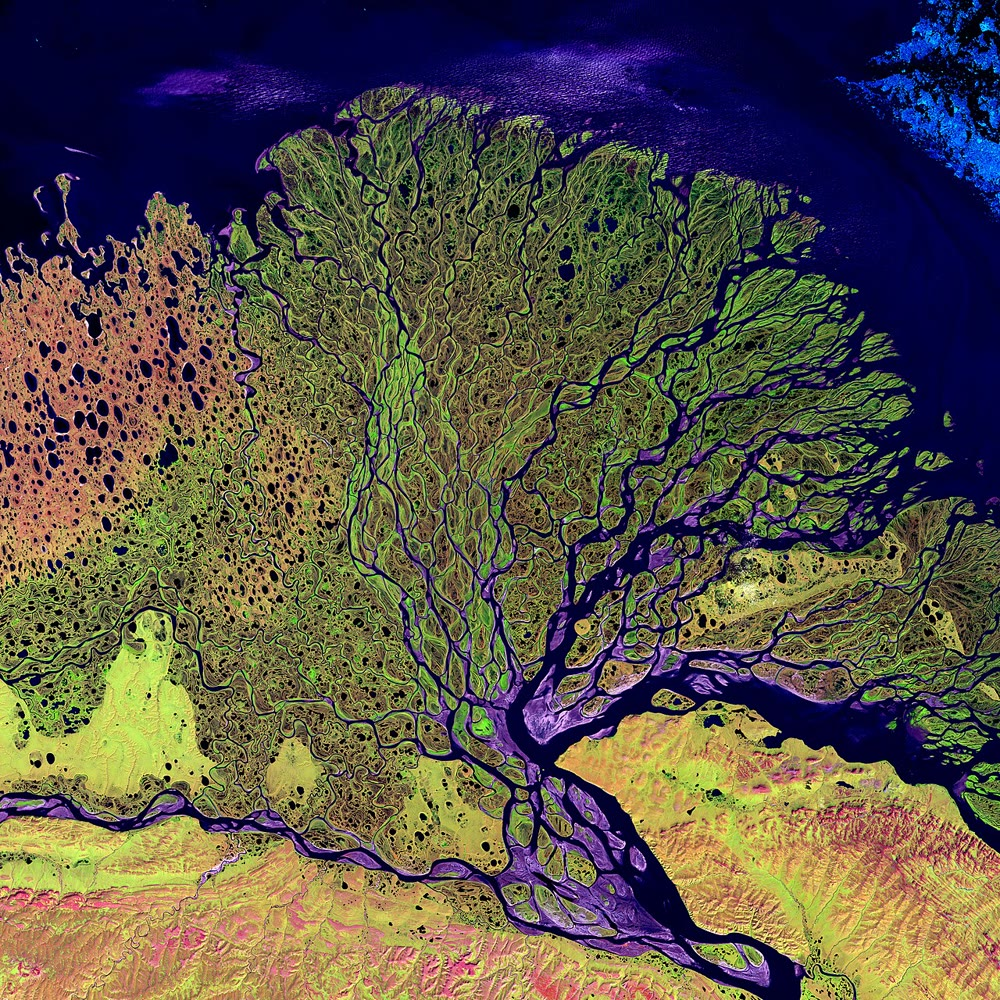
\includegraphics[width=\linewidth]{images/book1/g9-lena-delta.jpg}
\end{minipage}\hfill
\begin{minipage}[c]{0.46\linewidth}\raggedright
{\small साइबेरिया में लेना \omterm{def:g1:landscapes-around-us:water}{नदी} का \omterm{def:g5:water-shapes-the-land:delta}{डेल्टा}, जहाँ वह आर्कटिक \omterm{def:g2:water-on-earth:ocean}{महासागर} से मिलती है: 27~फ़रवरी
2000 का एक छद्म-रंग लैंडसैट चित्र, लघु-तरंग अवरक्त, अवरक्त और लाल प्रकाश से बना।
\omterm{def:g1:landscapes-around-us:water}{नदी} के अनेक धारा-मार्ग नीले दिखते हैं। USGS EROS डेटा केंद्र, NASA विज़िबल अर्थ के ज़रिए
(सार्वजनिक डोमेन,
विकिमीडिया कॉमन्स के ज़रिए)।}
\end{minipage}
% ledger: commons:lena-landsat
\label{fig:g9:maps-of-the-earth:lena}
\end{omfigure}

\section{उपग्रह स्थिति-निर्धारण}

कोई फ़ोन या कार पृथ्वी पर लगभग कहीं भी कुछ मीटर के भीतर बता सकती है कि वह कहाँ है। वह
उपग्रहों को देखती नहीं; उन्हें सुनती है।

\begin{definition}[उपग्रह स्थिति-निर्धारण]\label{def:g9:maps-of-the-earth:positioning}
\emph{उपग्रह स्थिति-निर्धारण}\index{उपग्रह स्थिति-निर्धारण} ऐसे कई उपग्रहों की दूरियों से
पृथ्वी पर कोई स्थिति ढूँढना है जिनकी स्थितियाँ ज्ञात हैं। अभिग्राही हर दूरी उस समय से निकालता है
जो उपग्रह के एक संकेत को उस तक पहुँचने में लगता
है।
\end{definition}

अमेरिकी प्रणाली, GPS, लगभग \qty{20200}{km} की ऊँचाई पर कम से कम 24 काम करते उपग्रह
रखती है। हर एक दिन में दो बार पृथ्वी की परिक्रमा करता है, ग्रह के चारों ओर फैली छह कक्षाओं में,
ताकि पृथ्वी के लगभग किसी भी बिंदु से कम से कम चार उपग्रह दिखाई दें। \qty{20200}{km} दूर
से प्रकाश की चाल से चलता एक संकेत $20\,200 \div
300\,000 \approx 0.067$~s
के बाद पहुँचता है: अभिग्राही यह समय मापता है और उसे एक दूरी में
बदलता
है।
% ledger: gps:constellation, const:c (travel time computed in figdata/grade-9/trilateration.py)

दूरियाँ स्थिति कैसे देती हैं? इस विचार को एक चपटे \omterm{def:g2:drawing-to-map:map}{मानचित्र} पर सोचो। अगर अभिग्राही बीकन~A से
\qty{5}{km} दूर है, तो वह A के चारों ओर \qty{5}{km} त्रिज्या के एक वृत्त पर कहीं है। अगर
वह B से भी \qty{10}{km} दूर है, तो वह दोनों वृत्तों पर है: उन दो बिंदुओं में से एक पर जहाँ वे
कटते हैं। एक तीसरी दूरी, C से \qty{5}{km}, सही बिंदु चुन लेती है। अंतरिक्ष में वृत्त गोले
बन जाते हैं, और इसी कारण से एक और उपग्रह की ज़रूरत होती
है।

\begin{omfigure}
\begin{minipage}[c]{0.5\linewidth}\centering
\begin{tikzpicture}
\begin{axis}[x=0.42cm, y=0.42cm, xmin=-1, xmax=13, ymin=-1.5, ymax=13,
  ticks=none, axis line style={black!40}]
  \addplot[omSea!70!black, line width=0.6pt] table {figdata/out/grade-9-trilateration-circles.dat};
  \addplot[only marks, mark=triangle*, mark size=2.6pt, point meta=explicit symbolic, nodes near coords,
    nodes near coords style={font=\footnotesize\bfseries, anchor=south west, inner sep=1pt}]
    table[meta=label] {figdata/out/grade-9-trilateration-beacons.dat};
  % labels first (on a white patch), then the points on top of them
  \addplot[only marks, mark=none, point meta=explicit symbolic, nodes near coords,
    nodes near coords style={font=\footnotesize\bfseries, anchor=north east, xshift=-1pt, yshift=-1pt, inner sep=1pt, fill=white, text=red!75!black}, skip coords between index={1}{2}]
    table[meta=label] {figdata/out/grade-9-trilateration-points.dat};
  \addplot[only marks, mark=none, point meta=explicit symbolic, nodes near coords,
    nodes near coords style={font=\footnotesize, anchor=south west, xshift=1pt, yshift=1pt, inner sep=1pt, fill=white}, skip coords between index={0}{1}]
    table[meta=label] {figdata/out/grade-9-trilateration-points.dat};
  \addplot[only marks, mark=*, mark size=2pt, red!75!black, skip coords between index={1}{2}] table {figdata/out/grade-9-trilateration-points.dat};
  \addplot[only marks, mark=o, mark size=2pt, fill=white, skip coords between index={0}{1}] table {figdata/out/grade-9-trilateration-points.dat};
\end{axis}
\end{tikzpicture}
\end{minipage}\hfill
\begin{minipage}[c]{0.46\linewidth}\raggedright
{\small एक चपटे \omterm{def:g2:drawing-to-map:map}{मानचित्र} पर स्थिति-निर्धारण (एक रेखाचित्र; किलोमीटर की जाली नहीं बनाई गई)।
अभिग्राही R, A से \qty{5}{km}, B से \qty{10}{km} और C से \qty{5}{km}
दूर है। A और B के चारों ओर के वृत्त R पर और एक झूठे बिंदु F पर कटते हैं; केवल
R ही C के चारों ओर के वृत्त पर भी है।}
\end{minipage}
% ledger: (invented region: exercise data, figdata/grade-9/trilateration.py)
\label{fig:g9:maps-of-the-earth:trilateration}
\end{omfigure}

\begin{omfigure}
\begin{minipage}[t]{0.48\linewidth}\centering
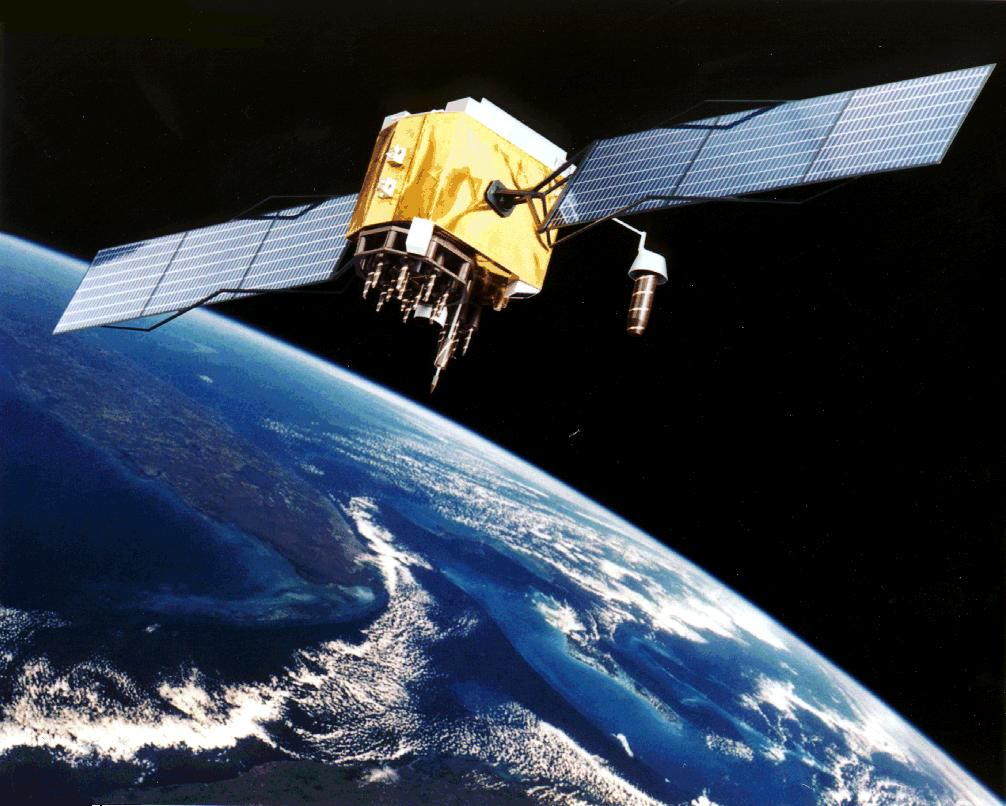
\includegraphics[width=\linewidth]{images/book1/g9-gps-satellite.jpg}

{\small कक्षा में एक GPS उपग्रह, जैसा एक कलाकार ने उसकी कल्पना की। NASA (सार्वजनिक
डोमेन, विकिमीडिया कॉमन्स के ज़रिए)।}
\end{minipage}\hfill
\begin{minipage}[t]{0.48\linewidth}\centering
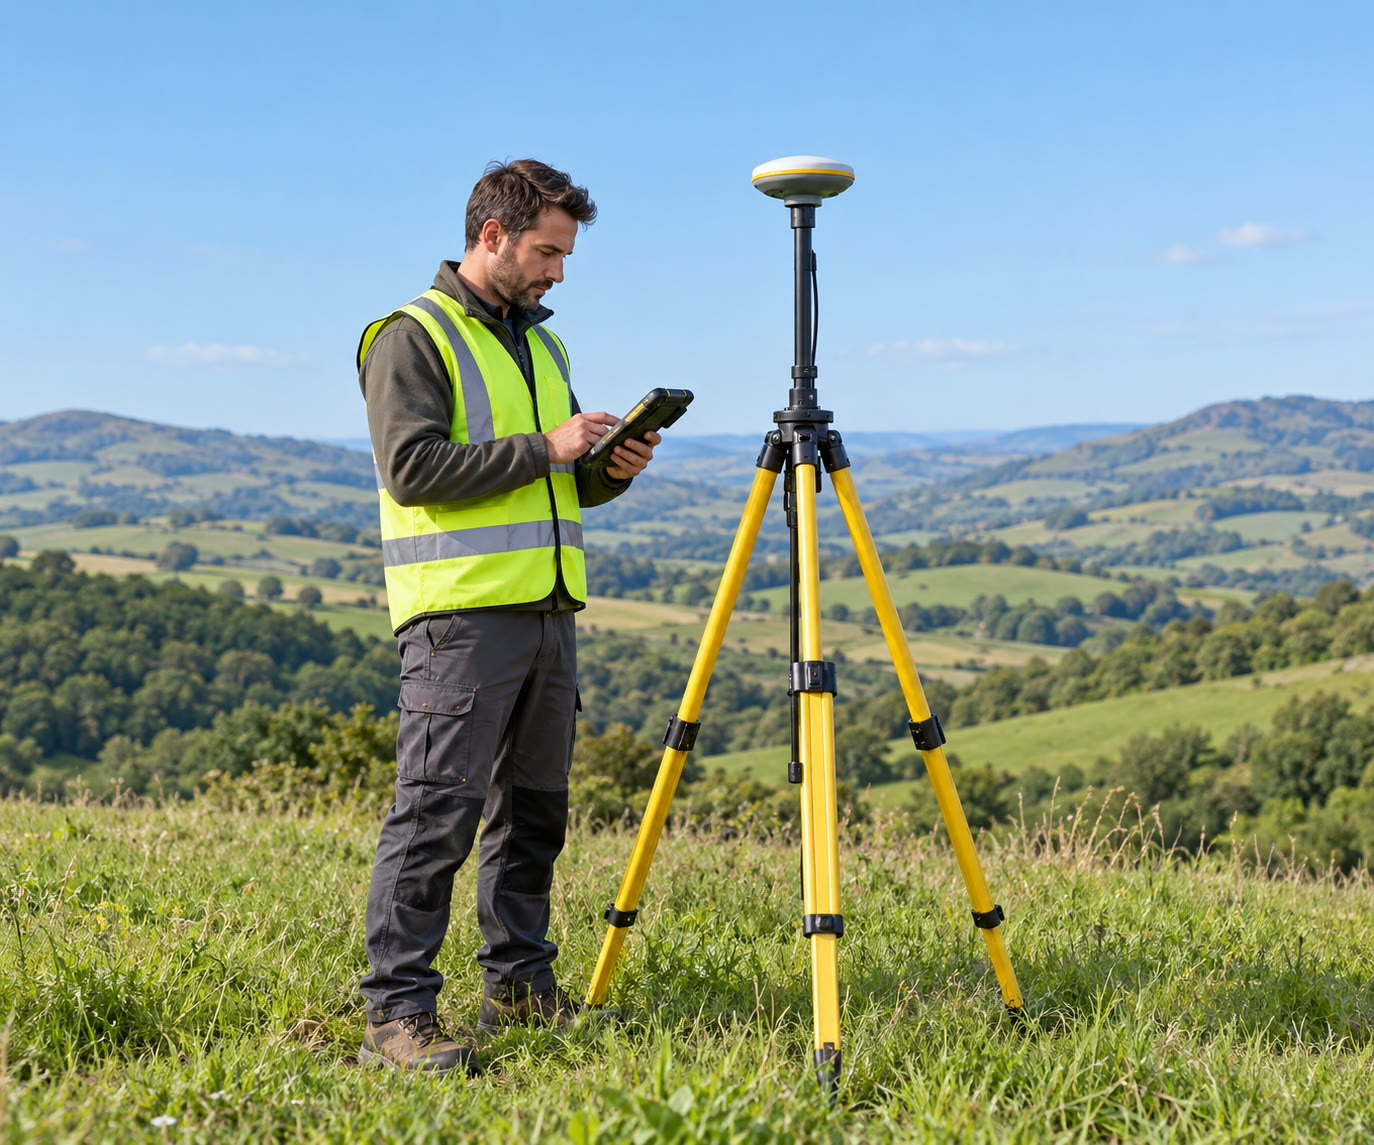
\includegraphics[width=\linewidth]{images/book1/ai/g9-surveyor.jpg}

{\small एक सर्वेक्षक तिपाई पर रखे उपग्रह अभिग्राही से किसी बिंदु की स्थिति तय करता है
(एक चित्रण)।}
\end{minipage}
% ledger: commons:gps-iif
\label{fig:g9:maps-of-the-earth:gps}
\end{omfigure}

\section{अभ्यास}

\begin{exercise}[$\star$]\label{exo:g9:maps-of-the-earth:1}
हर वर्णन के लिए शब्द बताओ। (क) एक नियम जो \omterm{def:g3:continents-and-oceans:globe}{ग्लोब} के हर बिंदु को एक चपटे \omterm{def:g2:drawing-to-map:map}{मानचित्र} के एक बिंदु
तक भेजता है। (ख) एक ही ऊँचाई वाले बिंदुओं को जोड़ने वाली रेखा। (ग) $1 : 50\,000$ जैसा
एक अनुपात। (घ) दो पड़ोसी \omterm{def:g9:maps-of-the-earth:contour}{समोच्च रेखाओं} के बीच ऊँचाई का अंतर। (ङ) दूरी से, उदाहरण के लिए
किसी उपग्रह से, पृथ्वी का
प्रेक्षण।
\end{exercise}

\begin{exercise}[$\star$]\label{exo:g9:maps-of-the-earth:2}
हर \omterm{def:g2:drawing-to-map:map}{मानचित्र} दूरी को ज़मीन की दूरी में, मीटर या किलोमीटर में, बदलो। (क) $1 : 25\,000$ के
\omterm{def:g2:drawing-to-map:map}{मानचित्र} पर \qty{4}{cm}। (ख) $1 : 50\,000$ के \omterm{def:g2:drawing-to-map:map}{मानचित्र} पर \qty{3}{cm}। (ग) $1 : 1\,000\,000$ के \omterm{def:g2:drawing-to-map:map}{मानचित्र} पर \qty{2.5}{cm}। (घ)
$1 : 25\,000$ के \omterm{def:g2:drawing-to-map:map}{मानचित्र} पर कितने सेंटीमीटर \qty{1}{km} दिखाते हैं?
\end{exercise}

\begin{exercise}[$\star$]\label{exo:g9:maps-of-the-earth:3}
सही या ग़लत? ग़लत वाक्यों को सुधारो। (क) कोई \omterm{def:g3:continents-and-oceans:world-map}{विश्व मानचित्र} बिना कुछ विकृत किए पूरी
पृथ्वी दिखा सकता है। (ख) मर्केटर \omterm{def:g2:drawing-to-map:map}{मानचित्र} पर ग्रीनलैंड जितना है उससे बड़ा दिखता है।
(ग) समक्षेत्र \omterm{def:g2:drawing-to-map:map}{मानचित्र} पर आकार हर जगह बने रहते हैं। (घ) कॉपी मशीन पर \omterm{def:g2:drawing-to-map:map}{मानचित्र} बड़ा
करने पर \omterm{def:g9:maps-of-the-earth:numerical-scale}{मापनी-पट्टी} सही रहती
है।
\end{exercise}

\begin{exercise}[$\star$]\label{exo:g9:maps-of-the-earth:4}
\omterm{def:g9:maps-of-the-earth:topographic-map}{स्थलाकृतिक मानचित्र} पर (क) \omterm{def:g9:maps-of-the-earth:contour}{समोच्च रेखाओं} के बहुत पास-पास होने का क्या अर्थ है? (ख) दूर-दूर
होने का? (ग) अंदर की ओर ऊँची होती बंद \omterm{def:g9:maps-of-the-earth:contour}{समोच्च रेखाएँ} क्या दिखाती हैं? (घ) दो \omterm{def:g9:maps-of-the-earth:contour}{समोच्च रेखाएँ}
कभी एक-दूसरे को क्यों नहीं काट सकतीं?
\end{exercise}

\begin{exercise}[$\star\star$]\label{exo:g9:maps-of-the-earth:5}
% ledger: data:ne-land (factor 1/cos^2, figdata/grade-9/projections.py)
मर्केटर \omterm{def:g2:drawing-to-map:map}{मानचित्र} पर, \omterm{def:g3:continents-and-oceans:equator}{भूमध्य रेखा} की तुलना में, \omterm{def:g6:latitude-longitude:latitude}{अक्षांश} \ang{60} पर क्षेत्रफल 4 गुना और
\omterm{def:g6:latitude-longitude:latitude}{अक्षांश} \ang{30} पर लगभग 1.33 गुना बढ़ाए जाते हैं। (क) \qty{1000}{km^2} की एक \omterm{def:g1:landscapes-around-us:water}{झील}
\ang{60} उत्तर पर \omterm{def:g2:drawing-to-map:map}{मानचित्र} पर बनाई जाती है। \omterm{def:g3:continents-and-oceans:equator}{भूमध्य रेखा} पर उसी आकार में बनी \omterm{def:g1:landscapes-around-us:water}{झील} का सच्चा
क्षेत्रफल क्या है? (ख) एक ही सच्चे क्षेत्रफल वाले दो द्वीप \ang{30} और \ang{60} पर हैं।
दूसरा पहले से कितने गुना बड़ा दिखता है? (ग) मर्केटर \omterm{def:g2:drawing-to-map:map}{मानचित्र} \omterm{def:g3:continents-and-oceans:poles}{ध्रुवों} को कभी क्यों नहीं दिखा
सकता?
\end{exercise}

\begin{exercise}[$\star\star$]\label{exo:g9:maps-of-the-earth:6}
% ledger: (invented region: the Varden Hills map of the chapter)
इस अध्याय में वार्डन पहाड़ियों का \omterm{def:g9:maps-of-the-earth:topographic-map}{स्थलाकृतिक मानचित्र} उपयोग करो। (क) \omterm{def:g9:maps-of-the-earth:contour}{समोच्च अंतराल} क्या है?
(ख) अपनी स्थानिक ऊँचाई से चिह्नित शिखर की ऊँचाई क्या है, और उसके ठीक चारों ओर की सूचक
\omterm{def:g9:maps-of-the-earth:contour}{समोच्च रेखा} की? (ग) \omterm{def:g1:landscapes-around-us:water}{नदी} पूर्व की ओर बहती है। \omterm{def:g1:landscapes-around-us:landform}{घाटी} का तल \omterm{def:g2:drawing-to-map:map}{मानचित्र} के पश्चिम में ऊँचा है या
पूर्व में? (घ) C--D के साथ, \omterm{def:g1:landscapes-around-us:water}{नदी} के उत्तर में, किन \omterm{def:g9:maps-of-the-earth:contour}{समोच्च रेखाओं} के बीच रेखाएँ सबसे पास-पास
हैं? इससे तुम्हें वहाँ की ढाल के बारे में क्या पता चलता
है?
\end{exercise}

\begin{exercise}[$\star\star$]\label{exo:g9:maps-of-the-earth:7}
% ledger: (invented region: profile C--D, figdata/grade-9/varden_topo.py)
इस अध्याय की परिच्छेदिका C--D का उपयोग करो। (क) C और D लगभग किस ऊँचाई पर हैं?
(ख) परिच्छेदिका के साथ सबसे कम ऊँचाई क्या है, और वह C से कितनी दूर है? (ग) C--D के साथ
समतल \omterm{def:g1:landscapes-around-us:landform}{घाटी} तल कितना लंबा है? (घ) परिच्छेदिका की ऊर्ध्वाधर मापनी तीन गुना खींचकर बनाई गई है।
मानचित्रकार अक्सर ऐसा क्यों करते
हैं?
\end{exercise}

\begin{exercise}[$\star\star$]\label{exo:g9:maps-of-the-earth:8}
$1 : 25\,000$ के \omterm{def:g2:drawing-to-map:map}{मानचित्र} पर एक रास्ता \qty{200}{m} की \omterm{def:g9:maps-of-the-earth:contour}{समोच्च रेखा} को और फिर
\qty{2}{cm} आगे \qty{300}{m} की \omterm{def:g9:maps-of-the-earth:contour}{समोच्च रेखा} को पार करता है। (क) ज़मीन पर दोनों
बिंदुओं के बीच क्षैतिज दूरी क्या है? (ख) रास्ता कितना ऊपर चढ़ता है? (ग) ढाल प्रतिशत में क्या
है? (घ) और आगे, ऊँचाई में \qty{100}{m} के अंतर वाली दो \omterm{def:g9:maps-of-the-earth:contour}{समोच्च रेखाएँ} \omterm{def:g2:drawing-to-map:map}{मानचित्र} पर
\qty{4}{cm} दूर हैं। वहाँ रास्ता ज़्यादा खड़ा है या ज़्यादा हल्का? कितना?
\end{exercise}

\begin{exercise}[$\star\star$]\label{exo:g9:maps-of-the-earth:9}
% ledger: usgs:landsat1
लैंडसैट~1 दिन में 14 बार पृथ्वी की परिक्रमा करता था और हर 18 दिनों पर उसी जगह के ऊपर से
गुज़रता था। (क) उसी जगह के ऊपर से दो बार गुज़रने के बीच उसने कितनी परिक्रमाएँ कीं? (ख) हर
परिक्रमा में 103 मिनट लगते थे। 14 परिक्रमाएँ घंटों में कितनी लंबी हैं? (ग) एक वर्ष काम
करने के लिए बना, उसे अपने प्रक्षेपण के साढ़े पाँच वर्ष बाद, 6~जनवरी 1978 को बंद किया गया।
उसने अपने नियोजित जीवन का कितना गुना काम किया? (घ) पृथ्वी की सतह का एक बदलाव बताओ जो
वर्षों के अंतर पर ली गई एक ही जगह की तस्वीरें दिखा सकती
हैं।
\end{exercise}

\begin{exercise}[$\star\star$]\label{exo:g9:maps-of-the-earth:10}
% ledger: gps:constellation, const:c
एक GPS उपग्रह लगभग \qty{20200}{km} दूर है; उसका संकेत लगभग \qty{300000}{km}
प्रति सेकंड से चलता है। (क) संकेत को पहुँचने में कितना समय लगता है? जवाब वैज्ञानिक संकेतन
में लिखो। (ख) अगर किसी अभिग्राही की घड़ी $1 \times 10^{-3}$~s ग़लत होती, तो उससे दूरी में
कितनी त्रुटि होती? (ग) इससे तुम्हें \omterm{def:g9:maps-of-the-earth:positioning}{उपग्रह स्थिति-निर्धारण} में इस्तेमाल होने वाली घड़ियों के बारे
में क्या पता चलता
है?
\end{exercise}

\begin{exercise}[$\star\star\star$]\label{exo:g9:maps-of-the-earth:11}
किलोमीटर की जाली वाले एक चपटे \omterm{def:g2:drawing-to-map:map}{मानचित्र} पर बीकन A $(0, 0)$ पर है और बीकन B
$(10, 0)$ पर। एक अभिग्राही A से \qty{6}{km} और B से \qty{8}{km}
दूर है। (क) दिखाओ कि बिंदु $(3.6, 4.8)$ A से \qty{6}{km} और B से
\qty{8}{km} दूर है। (ख) A और B से उतनी ही दूरियों पर एक और बिंदु बताओ। (ग) एक तीसरा
बीकन C $(0, 10)$ पर है, और अभिग्राही उससे लगभग \qty{6.3}{km} दूर है। दोनों में से
कौन-सा बिंदु अभिग्राही है? (घ) \omterm{def:g9:maps-of-the-earth:positioning}{उपग्रह स्थिति-निर्धारण} को कई उपग्रहों की ज़रूरत क्यों होती
है?
\end{exercise}

\begin{exercise}[$\star\star\star$]\label{exo:g9:maps-of-the-earth:12}
% ledger: data:ne-land (areas, figdata/grade-9/projections.py)
अफ़्रीका की मुख्य भूमि लगभग 29~मिलियन~\unit{km^2} घेरती है और ग्रीनलैंड लगभग
2.1~मिलियन~\unit{km^2}। (क) अफ़्रीका कितने गुना बड़ा है? (ख) मर्केटर \omterm{def:g2:drawing-to-map:map}{मानचित्र} पर,
ग्रीनलैंड के बीच के पास, लगभग \ang{72} उत्तर पर, क्षेत्रफल लगभग 10.5 गुना बढ़ाए जाते हैं।
ग्रीनलैंड का दिखने वाला क्षेत्रफल अनुमानित करो। (ग) अफ़्रीका \omterm{def:g3:continents-and-oceans:equator}{भूमध्य रेखा} के दोनों ओर फैला है,
जहाँ क्षेत्रफल थोड़ा ही बढ़ाए जाते हैं। (ख) के अपने जवाब की तुलना अफ़्रीका के क्षेत्रफल से
करो, और अध्याय की शुरुआत के दीवार \omterm{def:g2:drawing-to-map:map}{मानचित्र} को समझाओ। (घ) \omterm{def:g3:continents-and-oceans:continent}{महाद्वीपों} के आकार निष्पक्ष रूप
से दिखाने के लिए तुम कौन-सा प्रक्षेप चुनोगे?
\end{exercise}

\section{समस्या: वार्डन पहाड़ियों के पार एक पगडंडी}

\begin{problem}[{सप्ताहांत समस्या --- योजनाकारों ने स्थलाकृतिक मानचित्र पर वार्डन पहाड़ियों
के पार एक पगडंडी बनाई है; अंतिम उत्तर पगडंडी की किलोमीटर में लंबाई और मीटर में उसकी कुल
चढ़ाई है}]
\label{pb:g9:maps-of-the-earth:1}
% ledger: (invented region: the Varden Hills, figdata/grade-9/varden_topo.py, part problem: leg lengths 3.6 / 2.5 / 2.35 cm, spot heights 296 / 143 / 335 / 544 m, 4.2 km, 401 m)
पगडंडी एक खेत S से शुरू होती है, \omterm{def:g1:landscapes-around-us:water}{नदी} पर एक पुल B तक नीचे जाती है, फिर एक आश्रय W तक
चढ़ती है और आगे शिखर T तक। हर हिस्सा सीधा है और या तो केवल नीचे जाता है या केवल ऊपर। \omterm{def:g2:drawing-to-map:map}{मानचित्र}
$1 : 50\,000$ पर है; S, B, W और T की ऊँचाइयाँ उनके बगल में लिखी
हैं।

\begin{omfigure}
\begin{tikzpicture}
\begin{axis}[x=1.6cm, y=1.6cm, xmin=2, xmax=8, ymin=1.8, ymax=6.2, ticks=none,
  axis line style={black!60}, clip mode=individual]
  \addplot[contour] table {figdata/out/shared-region-contours.dat};
  \addplot[index contour] table {figdata/out/shared-region-index-contours.dat};
  \addplot[river] table {figdata/out/shared-region-river.dat};
  \addplot[only marks, mark=none, point meta=explicit symbolic, nodes near coords,
    nodes near coords align={center}, nodes near coords style={font=\tiny, fill=white, inner sep=0.6pt, text=omContour}]
    table[meta=label] {figdata/out/grade-9-varden_topo-labels.dat};
  \addplot[red!75!black, line width=1pt, dashed] table[x=x_km, y=y_km] {figdata/out/grade-9-varden_topo-path.dat};
  \addplot[only marks, mark=*, mark size=1.6pt, red!75!black, point meta=explicit symbolic, nodes near coords,
    nodes near coords align={right}, nodes near coords style={font=\scriptsize\bfseries, text=black, fill=white, fill opacity=0.8, text opacity=1, inner sep=1pt}]
    table[meta=label] {figdata/out/grade-9-varden_topo-points.dat};
  \coordinate (na) at (axis cs:8.35,5.4);
\end{axis}
\pic at (na) {northarrow};
\end{tikzpicture}

{\small वार्डन पहाड़ियों के \omterm{def:g9:maps-of-the-earth:topographic-map}{स्थलाकृतिक मानचित्र} पर पगडंडी S--B--W--T (यहाँ छोटा करके
दिखाया गया; $1 : 50\,000$ के मूल \omterm{def:g2:drawing-to-map:map}{मानचित्र} पर हिस्से 3.6, 2.5 और \qty{2.35}{cm}
मापते हैं)।}
\label{fig:g9:maps-of-the-earth:path}
\end{omfigure}

\noindent\textbf{भाग I --- मानचित्र पर मार्ग।}\par\nopagebreak
\begin{enumerate}[beginpenalty=10000]
  \item $1 : 50\,000$ पर \omterm{def:g2:drawing-to-map:map}{मानचित्र} का \qty{1}{cm} ज़मीन पर कितने मीटर
        दिखाता है?
  \item मूल \omterm{def:g2:drawing-to-map:map}{मानचित्र} पर हिस्सा S--B \qty{3.6}{cm} मापता है। ज़मीन पर वह किलोमीटर में
        कितना लंबा है?
  \item हिस्से B--W और W--T \qty{2.5}{cm} और \qty{2.35}{cm} मापते हैं।
        ज़मीन पर वे कितने लंबे हैं?
  \item B से T तक रास्ता मोटे तौर पर किस दिशा में चलता है?
\end{enumerate}

\noindent\textbf{भाग II --- चढ़ाई।}\par\nopagebreak
\begin{enumerate}[resume, beginpenalty=10000]
  \item \omterm{def:g2:drawing-to-map:map}{मानचित्र} का \omterm{def:g9:maps-of-the-earth:contour}{समोच्च अंतराल} क्या है?
  \item कौन-सा हिस्सा नीचे जाता है? कितने मीटर?
  \item B--W पर, और W--T पर, रास्ता कितने मीटर चढ़ता है?
  \item हिस्से W--T की औसत ढाल प्रतिशत में क्या है?
  \item योजनाकारों ने रास्ता S से T तक एक सीधी रेखा में क्यों नहीं
        बनाया?
\end{enumerate}

\noindent\textbf{भाग III --- सैर।}\par\nopagebreak
\begin{enumerate}[resume, beginpenalty=10000]
  \item मान लो कि एक पैदल यात्री समतल पर एक घंटे में \qty{4}{km} चलता है और हर
        \qty{10}{m} चढ़ाई के लिए एक मिनट और लेता है। पूरी सैर में कितना समय
        लगता है?
  \item एक दूसरी पैदल यात्री पगडंडी पर उलटी ओर, T से S तक, चलती है। वह कितने मीटर
        चढ़ती है?
  \item पगडंडी की कुल लंबाई किलोमीटर में, और उसकी कुल चढ़ाई मीटर में, क्या
        है?
\end{enumerate}
\end{problem}
